\documentclass[CJKutf8,dvipsnames,table]{beamer}
\usepackage{hyperref}
\hypersetup{
  pdfpagemode={FullScreen},
  colorlinks={true},
  linkcolor={blue},
}

%% https://tex.stackexchange.com/questions/47576/combining-ifxetex-and-ifluatex-with-the-logical-or-operation
\usepackage{iftex}
\newif\ifxetexorluatex % a new conditional starts as false
\ifnum 0\ifxetex 1\fi\ifluatex 1\fi>0
   \xetexorluatextrue
\fi
\usepackage{ifplatform}
\ifxetexorluatex
	\usepackage[slantfont,boldfont]{xeCJK}
	\ifwindows
		\setCJKmainfont{SimSun} % Windows默认中文字体:中易宋体
	\else
		\ifmacosx
			\setCJKmainfont{STSong} % MacOS默认中文字体:华文宋体
		\else
			\setCJKmainfont{Noto Serif CJK SC} % Linux默认中文字体:思源宋体(By Adobe & Google)
		\fi
	\fi
\else
	\usepackage{CJKutf8}
\fi

\usepackage[export]{adjustbox}

\usetheme{Madrid}%{Warsaw}
\usecolortheme{default}

\setbeamertemplate{footline}[page number]{} %gets rid of bottom navigation bars
\setbeamertemplate{navigation symbols}{} %gets rid of navigation symbols

\title{数字信号处理}
\subtitle{第2章:信号}
\author{洪明坚}
\institute{重庆大学软件学院}
\date{\today}

\begin{document}
\ifxetexorluatex\else
\begin{CJK*}{UTF8}{song}
\fi

  \AtBeginSection[]
  {
    \begin{frame}
      \frametitle{Outline}
      \tableofcontents[currentsection]
    \end{frame}
  }

  \frame{\titlepage}
  \frame{\frametitle{目录}\tableofcontents}
  
  \section{信号}
  
  %% PAGE
  \begin{frame}
    \frametitle{定义}
    \begin{itemize}
    \item 新华字典:一种可以觉察的物理量或脉冲(如电压、电流、磁场强度等),通过它们能传达消息或信息。
    \item 维基百科:A signal is a function that conveys information about the behavior of a system or attributes of some phenomenon.
    \item 例子
        \begin{itemize}
        \item 声音、温度、电压/电流、光强等等
        \end{itemize}    
    \end{itemize}
  \end{frame}
  
  %% PAGE
  \begin{frame}
    \frametitle{连续/离散时间信号} 
    主要考虑一维信号
    \begin{itemize}
    \item $x: I \to X$,其中$I \subset \mathbb{R}$,$X \subset \mathbb{R}$或$\mathbb{C}$
    \item 经常称自变量为``时间''
    \end{itemize}
    根据自变量的连续/离散属性,
    \begin{itemize}
    \item 连续时间信号:$I \subset \mathbb{R}$,用$x(t)$表示
        \begin{itemize}
        \item 如果$X$也是连续的,称为模拟({\color{red}A}nalog)信号
        \item 真实世界的信号大多为连续时间信号,如声音、温度等
        \end{itemize}
    \item 离散时间信号:$I \subset \mathbb{Z}$,用$x[n]$表示
        \begin{itemize}
        \item 如果$X$也是离散的,称为数字({\color{red}D}igital)信号
        \item 通过对连续时间信号进行采样,可以得到
        \end{itemize}
    \end{itemize}
  \end{frame}

  %% PAGE
  \begin{frame}
    \frametitle{模拟信号$\leftrightharpoons$数字信号} 
    \begin{itemize}
    \item A/D:模拟信号,对时间进行采样(Sample),再对取值进行量化(Quantize),得到数字信号
    \end{itemize}
	    \begin{center}
	    	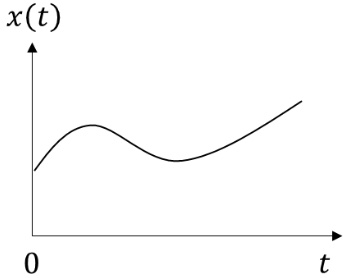
\includegraphics[scale=0.3]{contisignal}  
			\hspace{1mm}
	    	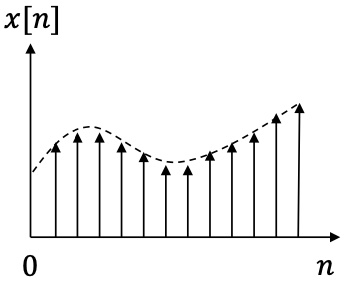
\includegraphics[scale=0.3]{samplesignal}  
			\hspace{1mm}
	    	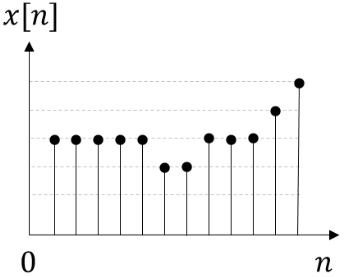
\includegraphics[scale=0.3]{discretesignal}    
	    \end{center}    
    \begin{itemize}
    \item D/A:可以用插值(Interpolate)进行恢复或重建
    \end{itemize}
	    \begin{center}
	    	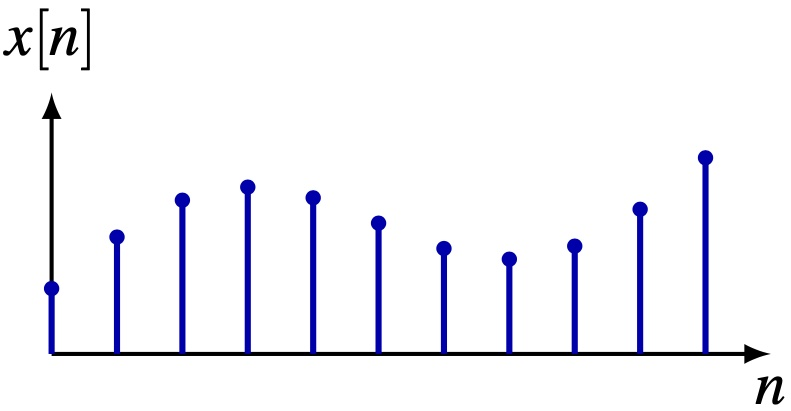
\includegraphics[scale=0.2]{dac1}  
			\hspace{1mm}
	    	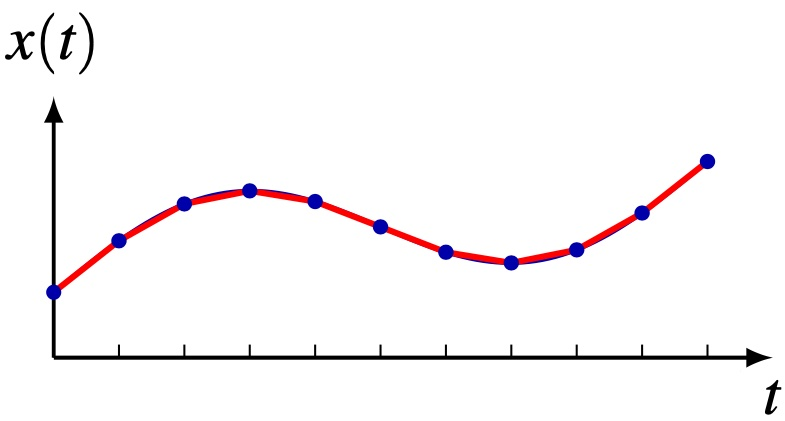
\includegraphics[scale=0.2]{dac2}  
	    \end{center}
  \end{frame}  

  %% PAGE
  \begin{frame}
    \frametitle{数字信号处理}
    \begin{itemize}
    \item 数字信号的处理
    \end{itemize}
    \begin{center}
      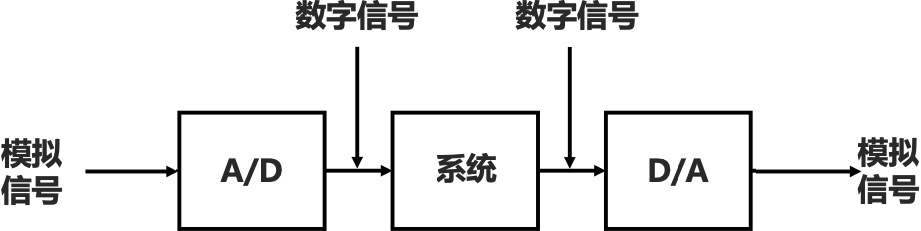
\includegraphics[scale=.3]{dsp}
    \end{center}
  \end{frame}
  
  %% PAGE
  \begin{frame}
    \frametitle{Questions}
    \begin{itemize}
    \item Any questions?
    \end{itemize}
    \begin{center}
      
\includegraphics[scale=.5]{question}
    \end{center}
  \end{frame}
  
  \section{信号的变换}
  
  %% PAGE
  \begin{frame}
    \frametitle{平移}
    \begin{itemize}
    \item 连续:$x(t) \rightarrow x(t-t_0)$
        \begin{itemize}
        \item 图中$t_0<0$,超前
        \end{itemize}
    \end{itemize}
    \begin{center}
      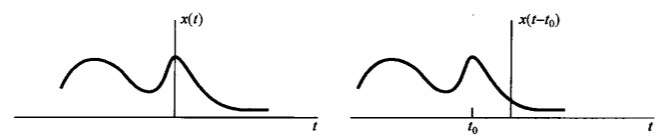
\includegraphics[scale=.4]{cshift}
    \end{center}
    \begin{itemize}
    \item 离散:$x[n] \rightarrow x[n-n_0]$    
        \begin{itemize}
        \item 图中$n_0>0$,延迟
        \end{itemize}
    \end{itemize}
    \begin{center}
      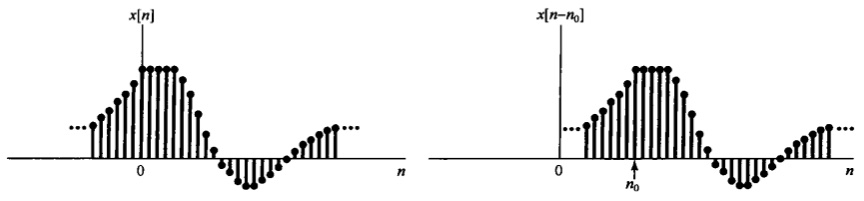
\includegraphics[scale=.3]{dshift}
    \end{center}
  \end{frame}  

  %% PAGE
  \begin{frame}
    \frametitle{翻转}
    \begin{itemize}
    \item 连续:$x(t) \rightarrow x(-t)$
    \end{itemize}
    \begin{center}
      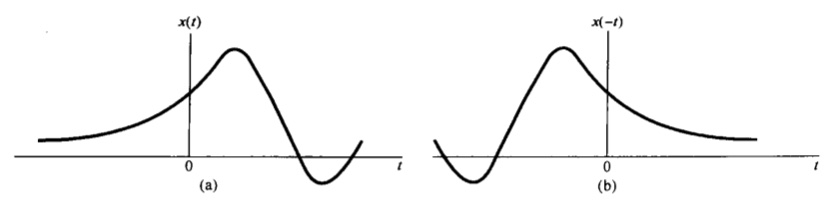
\includegraphics[scale=.4]{creversal}
    \end{center}
    \begin{itemize}
    \item 离散:$x[n] \rightarrow x[-n]$    
    \end{itemize}
    \begin{center}
      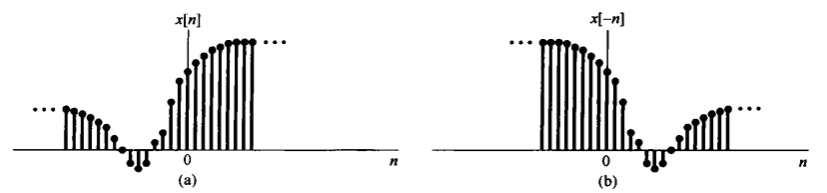
\includegraphics[scale=.4]{dreversal}
    \end{center}
  \end{frame}  

  %% PAGE
  \begin{frame}
    \frametitle{伸缩}
    \begin{itemize}
    \item 连续:$x(t) \rightarrow x(\alpha t), \alpha > 0$
    \end{itemize}
    \begin{center}
      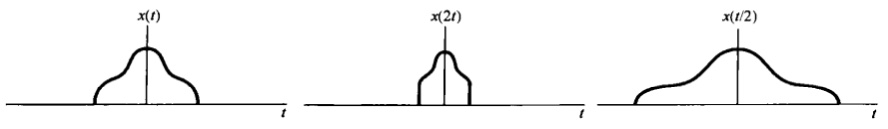
\includegraphics[scale=.4]{cscale}
    \end{center}
    \begin{itemize}
    \item 离散:$x[n] \rightarrow x[kn], k > 0$    
        \begin{itemize}
        \item $k>1$,下采样(Downsampling),也称为抽取(Decimation)
        \item $k<1$,上采样(Upsampling),可能需要插值
        \end{itemize}   
    \end{itemize} 
    \begin{center}
      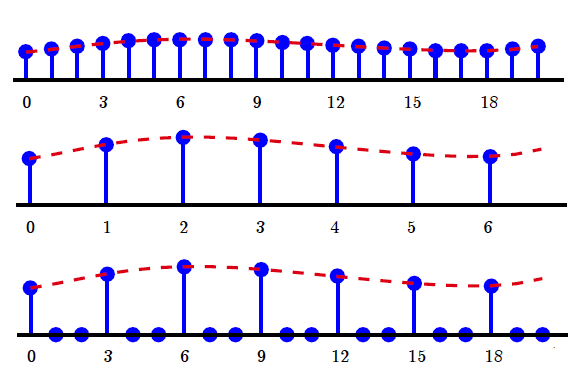
\includegraphics[scale=.28]{dscale}
    \end{center}    
  \end{frame}  

  %% PAGE
  \begin{frame}
    \frametitle{奇偶分解}
    \begin{itemize}
    \item 奇信号:$x(-t)=-x(t), x[-n]=-x[n]$
    \item 偶信号:$x(-t)=x(t), x[-n]=x[n]$
    \item 奇偶分解:任意信号都可以分解为一个奇信号和一个偶信号之和
    \begin{itemize}
    \item $x(t)=Od(x)+Ev(x)$。其中,$Od(x)=\frac{1}{2}[x(t)-x(-t)]$, $Ev(x)=\frac{1}{2}[x(t)+x(-t)]$,
    \end{itemize}
    \end{itemize}
    \begin{center}
      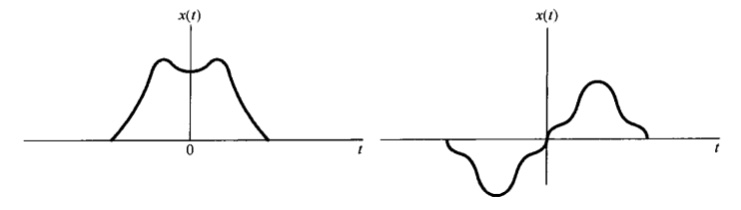
\includegraphics[scale=.4]{odev}
    \end{center}       
  \end{frame}  
  
  %% PAGE
  \begin{frame}
    \frametitle{Questions}
    \begin{itemize}
    \item Any questions?
    \end{itemize}
    \begin{center}
      
\includegraphics[scale=.5]{question}
    \end{center}
  \end{frame}

  \section{信号的能量与功率}
  
  %% PAGE
  \begin{frame}
    \frametitle{能量与功率}
    \begin{itemize}
    \item 连续
        \begin{itemize}
        \item 总能量:$E=\int_{-\infty}^{\infty} |x(t)|^2 \,dt$
        \item 平均功率:$P=\lim_{T\to\infty} \int_{-T}^{T} |x(t)|^2 \,dt $
        \end{itemize}
    \end{itemize}
    \begin{itemize}
    \item 离散   
        \begin{itemize}
        \item 总能量:$E=\sum_{n=-\infty}^{\infty}|x[n]|^2$
        \item 平均功率:$P=\lim_{N\to\infty}\frac{1}{2N+1}\sum_{n=-N}^{N}|x[n]|^2$
        \end{itemize}
    \item 能量信号:能量有限
        \begin{itemize}
        \item 即$E<\infty$,则$P=0$
        \end{itemize}
    \item 功率信号:功率有限
        \begin{itemize}
        \item 即$0<P<\infty$,则$E\to\infty$
        \end{itemize}
    \item 思考
        \begin{itemize}
        \item $x(t)=sin(t)$是什么信号?
        \item $x(t)=t$是什么信号?
        \end{itemize}
    \end{itemize}
  \end{frame}  
  
  \section{常用的信号}
  
  %% PAGE
  \begin{frame}
    \frametitle{常用的信号}
    \begin{itemize}
    \item 单位阶跃信号
    \item 单位冲激信号   
    \item 周期信号
    \item 指数信号和正弦信号
    \end{itemize}
  \end{frame}  

  %% PAGE
  \begin{frame}
    \frametitle{单位阶跃信号}
    \begin{itemize}
    \item Unit step function
    \begin{itemize}
    \item 也称为Heaviside step function
    \end{itemize}    
    
	\begin{tabular}{ll}
	\raisebox{-.5\height}

    连续:
    \begin{math}
u(t) = 
\left\{
    \begin {aligned}
         & 0 \quad & t < 0 \\
         & 1 \quad & t \geq 0                  
    \end{aligned}
\right.
	\end{math}

&
    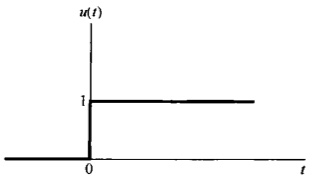
\includegraphics[valign=m,scale=.3]{cunitstepfunction}    \\
    \end{tabular}    

	\begin{tabular}{ll}
	\raisebox{-.5\height}

    离散:
    \begin{math}
u[n] = 
\left\{
    \begin {aligned}
         & 0 \quad & n < 0 \\
         & 1 \quad & n \geq 0                  
    \end{aligned}
\right.
	\end{math}

&
    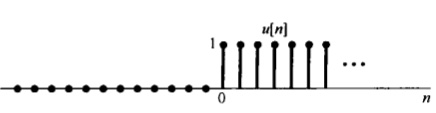
\includegraphics[valign=m,scale=.4]{dunitstepfunction}    \\
    \end{tabular}   

    \end{itemize}
  \end{frame}  

  %% PAGE
  \begin{frame}
    \frametitle{单位冲激信号}
    \begin{itemize}
    \item Unit impulse function
    \begin{itemize}
    \item 也称为Dirac delta function或$\delta$ function
    \end{itemize}  
     
	\begin{tabular}{ll}
	\raisebox{-.5\height}

    连续:
    \begin{math}
	\delta(t) = 0, t \neq 0; \int_{-\infty}^{\infty}\delta(t)dt=1 
	\end{math}

&
    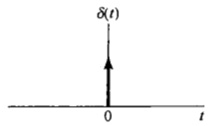
\includegraphics[valign=m,scale=.4]{cdelta}    \\
    \end{tabular}   

	\begin{tabular}{ll}
	\raisebox{-.5\height}

    离散:$\delta[n]=u[n]-u[n-1]$	

&
    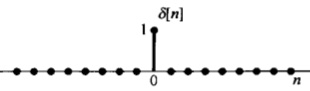
\includegraphics[valign=m,scale=.4]{ddelta}    \\
    \end{tabular}   
    
    \begin{itemize}
    \item 反过来,有$u[n]=\sum_{m=-\infty}^{n}\delta[m]$   
    \end{itemize}
    
	\item 具有采样功能
	\begin{itemize}
	\item 连续:对于任意$t_0$,有$x(t)\delta(t-t_0)=x(t_0)\delta(t-t_0)$
	\item 离散:对于任意$n_0$,有$x[n]\delta[n-n_0]=x[n_0]\delta[n-n_0]$
	\end{itemize}
    \end{itemize}
  \end{frame}

  %% PAGE
  \begin{frame}
    \frametitle{单位冲激信号(续)}
    \begin{itemize}
    \item
	\begin{tabular}{ll}
	\raisebox{-.5\height}

    设$u_{\Delta}(t)$=

&
    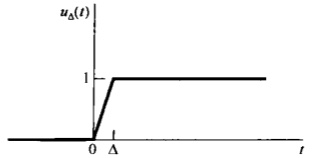
\includegraphics[valign=m,scale=.4]{uDelta}    \\
    \end{tabular}       
    

	\begin{tabular}{ll}
	\raisebox{-.5\height}

    则$\delta_{\Delta}(t)=\frac{du_{\Delta}(t)}{dt}$

&
    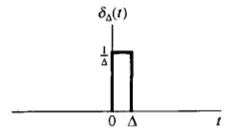
\includegraphics[valign=m,scale=.4]{deltaDelta}    \\
    \end{tabular}       
    
    \item 定义:$\delta(t)=\lim_{\Delta\to 0}\delta_{\Delta}(t)=\frac{du(t)}{dt}$
    \begin{itemize}
    \item 反过来,有$u(t)=\int_{-\infty}^{t}\delta(\tau)d\tau=\int_{0}^{\infty}\delta(t-\sigma)d\sigma$
    \end{itemize}
    \end{itemize}
  \end{frame}

  %% PAGE
  \begin{frame}
    \frametitle{Questions}
    \begin{itemize}
    \item Any questions?
    \end{itemize}
    \begin{center}
      
\includegraphics[scale=.5]{question}
    \end{center}
  \end{frame}
  
  %% PAGE
  \begin{frame}
    \frametitle{周期信号}
    \begin{itemize}
    \item 连续:
    \begin{itemize}
    \item 存在一个$T>0$,对任意的$t$,有$x(t)=x(t+T)$,则称$x(t)$是周期为$T$的周期(periodic)信号
    \begin{itemize}
    \item 如果不存在这样的T,则$x(t)$是非周期(aperiodic)信号
    \end{itemize}
    \item 使$x(t)=x(t+T)$成立的最小的$T=T_0$,称为基波周期(fundamental period)
    \end{itemize}
    \item 离散:
    \begin{itemize}
    \item 存在一个正整数$N$,对任意的$n$,有$x[n]=x[n+N]$
    \end{itemize}
    \end{itemize}
  \end{frame}  
  
  %% PAGE
  \begin{frame}
    \frametitle{指数信号和正弦信号}
    \begin{itemize}
    \item 复指数信号$x(t)=Ae^{at}, A/a \in \mathbb{C}$
    \item 当$A, a \in \mathbb{R}$时,
    \end{itemize}
    \begin{center}
      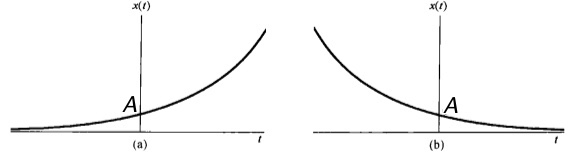
\includegraphics[scale=.4]{cexp}
    \end{center}  
  \end{frame}  
  
  %% PAGE
  \begin{frame}
    \frametitle{指数信号和正弦信号}
    \begin{itemize}
    \item 当$A \in \mathbb{R}$、$a$是纯虚数,即$a=j\omega_0$,$x(t)=Ae^{j\omega_{0}t}$是周期函数
    \begin{itemize}
    \item $e^{j\omega_{0}t}=e^{j\omega_{0}(t+T)} \Rightarrow e^{j\omega_{0}T}=1 \Rightarrow \omega_0 T=2\pi k, k \in \mathbb{Z}$
    \item 当$\omega_0 \neq 0$时,$T_0=\frac{2\pi}{|\omega_0|}$
    \item 当$\omega_0=0$时,$T_0$可以是任何值
    \end{itemize}
    \item 根据欧拉公式:$x(t)=Ae^{j\omega_0 t}=Acos(\omega_0 t)+jAsin(\omega_0 t)$
    \end{itemize}
    \begin{center}
      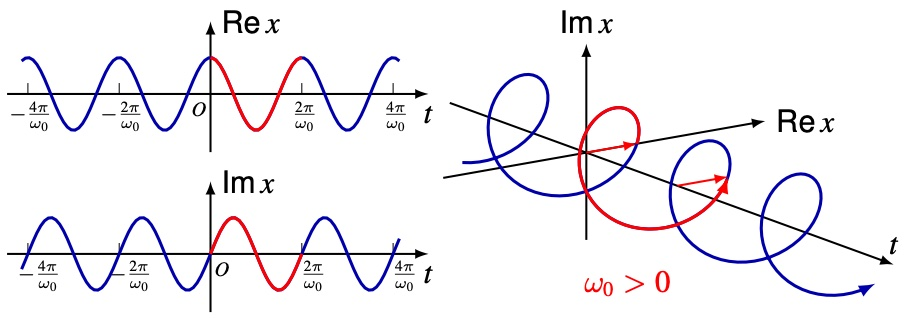
\includegraphics[scale=.4]{csinusoid}
    \end{center}     
  \end{frame}    

  %% PAGE
  \begin{frame}
    \frametitle{指数信号和正弦信号}
    \begin{itemize}
    \item 正弦(sinusoidal)信号:$x(t)=Acos(\omega_0 t + \phi)$
    \item 根据欧拉公式:$Acos(\omega_0 t + \phi)=\frac{A}{2}e^{j\phi}e^{j\omega_0 t}+\frac{A}{2}e^{j\phi}e^{-j\omega_0 t}$
    \end{itemize}
    \begin{center}
      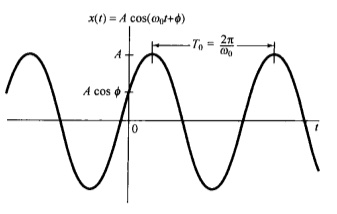
\includegraphics[scale=.5]{ccossinusoid}
    \end{center}  
  \end{frame} 

  %% PAGE
  \begin{frame}
    \frametitle{指数信号和正弦信号}
    \begin{itemize}
    \item 当$A, a \in \mathbb{C}$时,用极坐标表示$A=|A|e^{j\theta}$,用笛卡尔坐标表示$a=r+j\omega_0$
    \begin{itemize}
    \item 则$x(t)=Ae^{at}=|A|e^{rt}e^{j(\omega_0 t+\theta)}$
    \\ $=|A|e^{rt}cos(\omega_0 t + \theta)+j|A|e^{rt}sin(\omega_0 t + \theta)$
    \item 这种具有指数衰减振幅的正弦信号称为阻尼正弦振荡(damped sinusoids)函数
    \end{itemize}
    \end{itemize}
    \begin{center}
      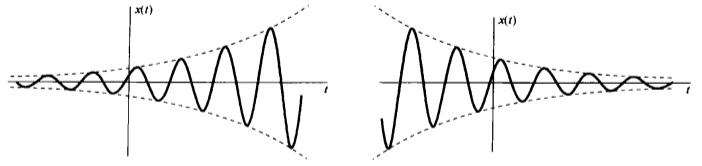
\includegraphics[scale=.5]{dampedsinusoids}
    \end{center}  
  \end{frame} 

  %% PAGE
  \begin{frame}
    \frametitle{指数信号和正弦信号}
    \begin{itemize}
    \item 离散的$x[n]=e^{j\omega_0 n}$与连续的$x(t)=e^{j\omega_{0}t}$相比,有两个重要区别
        \begin{itemize}
        \item 1、$x(t)$的频率随着$\omega_0$的增加而增大;然而,由$e^{j(\omega_0 + 2k\pi)n}=e^{j2k\pi n}e^{j\omega_0 n}=e^{j\omega_0 n}$,频率为$\omega_0$的$x[n]$与$(\omega_0 +2k\pi)$的$x[n]$完全相同。
        因此,对于$x[n]=e^{j\omega_0 n}$,仅需考虑某一个$2\pi$区间内选择$\omega_0$即可,如$[0, 2\pi)$或$[-\pi, \pi)$
        \end{itemize}    
    \end{itemize}
    \begin{center}
      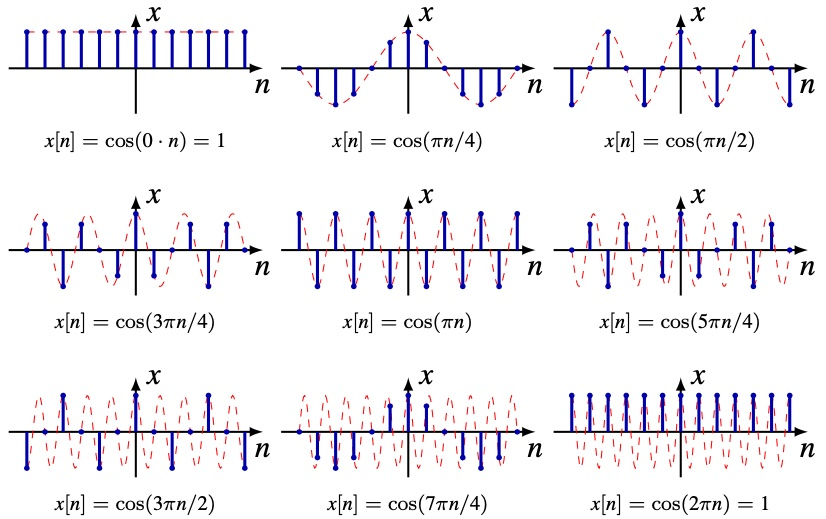
\includegraphics[scale=.3]{dsinusoidp1}
    \end{center}  
  \end{frame} 

  %% PAGE
  \begin{frame}
    \frametitle{指数信号和正弦信号}
    \begin{itemize}
    \item 离散的$x[n]=e^{j\omega_0 n}$与连续的$x(t)=e^{j\omega_{0}t}$相比,有两个重要区别
        \begin{itemize}
        \item 2、对于任何$\omega_0$,$x(t)$都是周期的;而$x[n]$是周期的仅当$e^{j\omega_0 (n + N)}=e^{j\omega_0 n} \Rightarrow e^{j\omega_0 N}=1 \Rightarrow \omega_0 N=2\pi m, m \in \mathbb{Z}$,即$\frac{\omega_0}{2\pi}$是有理数时
		\begin{itemize}
		\item 比如,$x[n]=cos(2\pi n /12)$是周期的,而$x[n]=cos(n/6)$不是周期的
		\end{itemize}
        \end{itemize}    
    \end{itemize}
  \end{frame} 
    
  %% PAGE
  \begin{frame}
    \frametitle{Questions}
    \begin{itemize}
    \item Any questions?
    \end{itemize}
    \begin{center}
      
\includegraphics[scale=.5]{question}
    \end{center}
  \end{frame}    
    
\ifxetexorluatex\else
\end{CJK*}
\fi
\end{document}

%%% Local Variables: 
%%% mode: latex
%%% TeX-master: t
%%% End: 
